\begin{exercice}
   Le triangle ci-dessous a été réalisé à main levée.\\
   Construire ce triangle avec les instruments de géométrie en respectant les mesures indiquées.\\
   Puis placer le point $L$ milieu de $[IJ]$, tracer le segment $[LK]$ et mesurer la longueur de ce segment.
   \begin{center}
      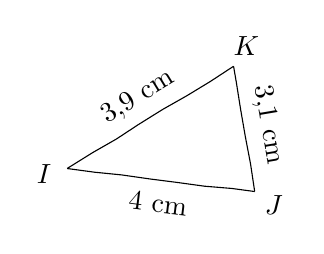
\begin{tikzpicture}[baseline,scale = 0.6]
      
         \tikzset{
            point/.style={
            thick,
            draw,
            cross out,
            inner sep=0pt,
            minimum width=5pt,
            minimum height=5pt,
            },
         }
         \draw [color={black}] (1.9241576315800704,-0.740011762630956) node[anchor = center, rotate = -7] {4 cm};
         \draw [color={black}] (4.239548494769968,0.9215481363489421) node[anchor = center, rotate = -80.42] {3,1 cm};
         \draw [color={black}] (1.4996967895932571,1.5081402749683903) node[anchor = center, rotate = 31.56] {3,9 cm};
         \draw[color ={black},decorate,decoration={random steps , amplitude = 0.3pt}] (0,0)--(3.970184606565288,-0.4874773736205899);
         \draw[color ={black},decorate,decoration={random steps , amplitude = 0.3pt}] (3.970184606565288,-0.4874773736205899)--(3.522845342799672,2.164225240012434);
         \draw[color ={black},decorate,decoration={random steps , amplitude = 0.3pt}] (3.522845342799672,2.164225240012434)--(0,0);      
         \draw [color={black}] (-0.48793262053547704,-0.10918680239562917) node[anchor = center,scale=1] {$I$};
         \draw [color={black}] (4.377756817413083,-0.7771062619322378) node[anchor = center,scale=1] {$J$};
         \draw [color={black}] (3.791956915116092,2.5856264284841615) node[anchor = center,scale=1] {$K$};   
      \end{tikzpicture}
   \end{center}
   \hrefMathalea{https://coopmaths.fr/mathalea.html?ex=6G21-2,s=4,s2=false,n=1&v=l}
\end{exercice}
 
\begin{corrige}
   Voici la construction que tu devais réaliser.\\
   Pour cette construction, nous avons utilisé le compas et la règle graduée.\\
   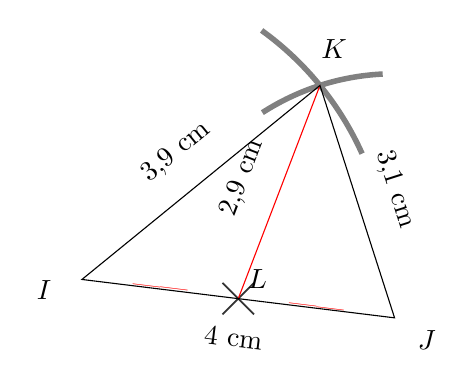
\begin{tikzpicture}[baseline]
      \tikzset{
         point/.style={
           thick,
           draw,
           cross out,
           inner sep=0pt,
           minimum width=5pt,
           minimum height=5pt,
         },
      }
      \draw[color={gray},line width = 2] (3.5576328090253835,1.5978888560053748) arc (24.19:54.19:3.900000000000001) ;
      \draw[color={gray},line width = 2] (3.8190819973235213,2.608837856048433) arc (92.79:122.79:3.1000000000000005) ;
      \draw [color={black}] (1.9241576315800704,-0.740011762630956) node[anchor = center, rotate = -7] {4 cm};
      \draw [color={black}] (3.972596041397484,1.141170588641989) node[anchor = center, rotate = -72.21] {3,1 cm};
      \draw [color={black}] (1.1954963585777292,1.6196568947241237) node[anchor = center, rotate = 39.19] {3,9 cm};
      \draw (1.985092303282644,-0.24373868681029495) node[above right] {$L$};
      \draw[color ={{black}},line width = 0.6666666666666666,opacity = 0.8] (1.785092303282644,-0.04373868681029494)--(2.185092303282644,-0.44373868681029494);
      \draw[color ={{black}},line width = 0.6666666666666666,opacity = 0.8] (1.785092303282644,-0.44373868681029494)--(2.185092303282644,-0.04373868681029494);
      \draw[color ={red}] (1.985092303282644,-0.24373868681029495)--(3.022845342799672,2.464225240012434);
      \draw [color={red}] (2.977638454923966,-0.3656080302154424) node[anchor = center, rotate = -7] {||};
      \draw [color={red}] (0.992546151641322,-0.12186934340514748) node[anchor = center, rotate = -7] {||};
      \draw [color={black}] (2.0370784908303428,1.2891662144488327) node[anchor = center, rotate = 69.03] {2,9 cm};
      \draw[color={black}] (0,0)--(3.970184606565288,-0.4874773736205899)--(3.022845342799672,2.464225240012434)--cycle;
      \draw [color={black}] (-0.48114647546232403,-0.1360076069570494) node[anchor = center,scale=1] {$I$};
      \draw [color={black}] (4.379921358495372,-0.7740359088586543) node[anchor = center,scale=1] {$J$};
      \draw [color={black}] (3.2017682806474355,2.9311155722232485) node[anchor = center,scale=1] {$K$};
   \end{tikzpicture}
   
   {\red Auto-vérification : le segment $[LK]$ mesure environ 2,9 cm}.
\end{corrige}
